\documentclass{article}
\usepackage{graphicx}
\usepackage{caption}
\usepackage{subcaption}
\usepackage{textcomp }

\graphicspath{{img/}}

\begin{document}
\section{Clustering}
We now run and compare some clustering algorithm in order to find some structures among the data. First we start with a basic \emph{K-Means} followed with some \emph{Hierarchical clustering techniques} and \emph{DBSCAN}. 
\subsection{Preprocessing}
The data matrix was first standardized and then the two principal components were extracted. The choice was between two and tree principal component since they retain respectively $\sim$0.65 and $\sim$0.8 of the variance of the data.

We selected the two principal components because it performed better on K-Means and in this way a visual inspection was possible.

\begin{figure}[h!]
    \centering
    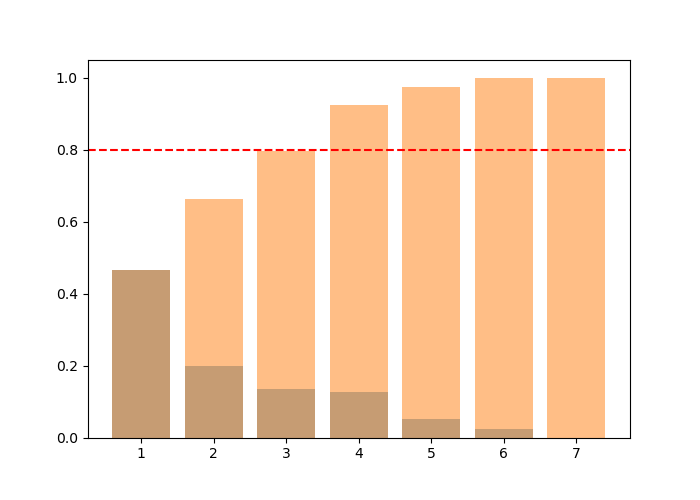
\includegraphics[scale=0.4]{pca.png}
    \caption{Explained variance ratio}
    \label{fig:pca_img}
\end{figure}

\subsection{K-Means}
The algorithm run for K ranging from two to ten clusters. For each iteration the SSE and the average silhouette value were computed.

\begin{figure}[h!]
     \centering
     \begin{subfigure}{0.49\textwidth}
         \centering
         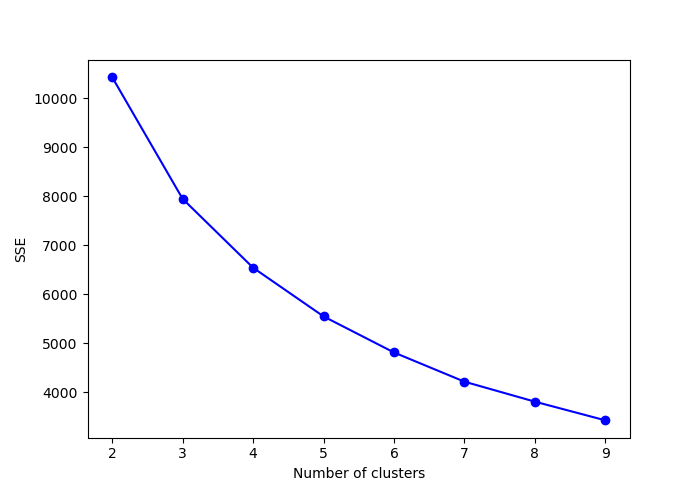
\includegraphics[scale=0.4]{sse.png}
         \caption{SSE}
         \label{fig:sse_img}
     \end{subfigure}
     \begin{subfigure}{0.49\textwidth}
         \centering
         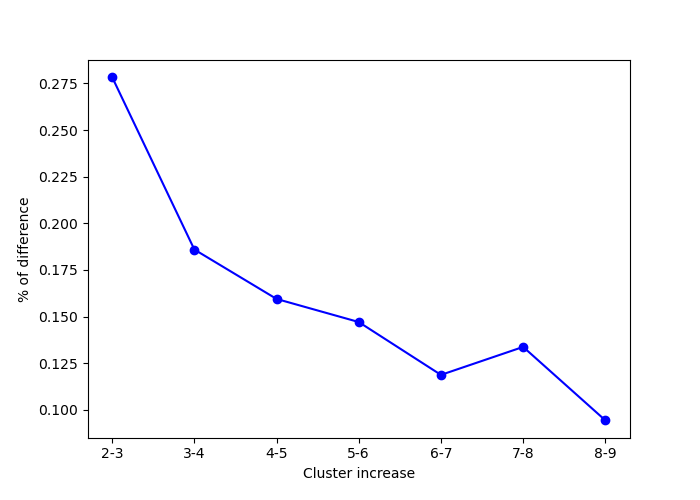
\includegraphics[scale=0.4]{perc.png}
         \caption{Percentage of decrease in SSE}
         \label{fig:pdiff_img}
     \end{subfigure}
     
     \begin{subfigure}{0.49\textwidth}
         \centering
         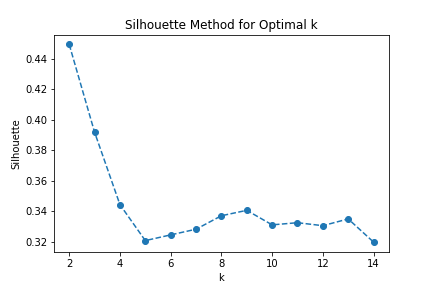
\includegraphics[scale=0.4]{sil.png}
         \caption{Average silhouette}
         \label{fig:sil_img}
     \end{subfigure}
     \caption{\emph{K-Means} metrics}
    \label{fig:km_metrics}
\end{figure}

By looking at the plots in Figure \ref{fig:km_metrics} we can see that there isn't a prominent \emph{elbow shape} so to get the optimal number of clusters the analysis of more metrics was necessary. At first we saw that for K moving from two to three the difference of the SSE in percentage was quite high ($\sim$0.3) while for all the other values the difference was below the 0.2, meaning that the most of the decrease in the SSE was in moving from 2 to 3 clusters. By inspecting the silhouette score it's possible to see that it has its maximum for K equal to two, followed by K equal to 3. In conclusion we opted of K equal to three to get a trade off between high silhouette and low SSE.

\begin{figure}[h!]
    \centering
    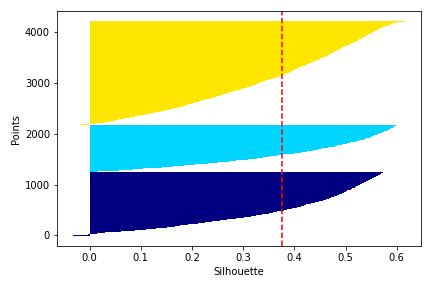
\includegraphics[scale=0.4]{sil_tot.png}
    \caption{Silhouette score for each data point. Each different color represent a different cluster, the dotted red line is the average silhouette coefficient.}
    \label{fig:silhouette}
\end{figure}

The resulting clusters have a comparable number of points. In particular the cluster zero has 1312 points, the cluster one 757 and the cluster two 2131. By looking at the plot of the Silhouette score (Figure \ref{fig:silhouette}) we see that a small fraction of points in cluster one and two have a negative value but overall the Silhouette suggest a good clustering.

\begin{figure}[h!]
    \centering
    \begin{subfigure}{0.49\textwidth}
        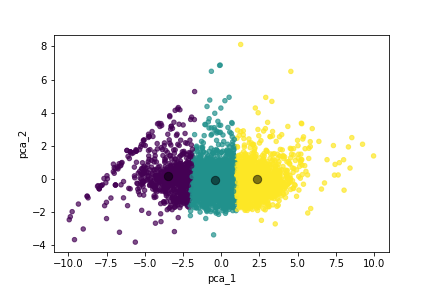
\includegraphics[width=\linewidth]{km_clusters.png}
        \caption{Clustering result}
        \label{fig:skmclust}
    \end{subfigure}
    \begin{subfigure}{0.49\textwidth}
        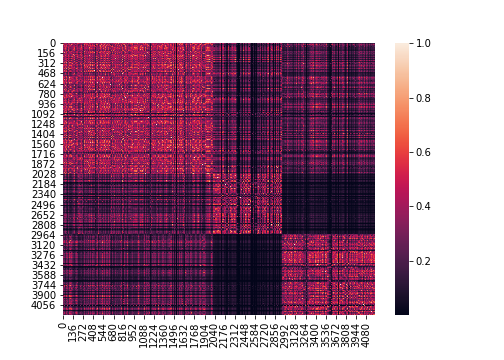
\includegraphics[width=\linewidth]{sim_heatmap.png}
        \caption{Similarity heatmap}
        \label{fig:sim_heatmap}
    \end{subfigure}
    
    \begin{subfigure}{0.49\textwidth}
        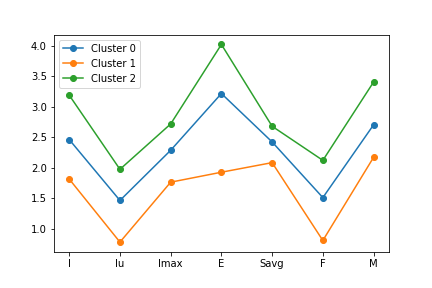
\includegraphics[width=\linewidth]{cluster_avg.png}
        \caption{The plot shows the average values for each attribute divided by the clusters. In particular is possible to see that \emph{Cluster 0} contains the most frequent and spending customers, followed by \emph{Cluster 2} and \emph{Cluster 1}}
        \label{fig:km_avg}
    \end{subfigure}
\end{figure}

The similarity matrix (Figure \ref{fig:sim_heatmap}) shows that the points within the same cluster are similar to each other when similarity is measure with $e^{-d(x, y)}$ where $x$ and $y$ are data points and $d$ is the euclidean distance. In particular the cluster 0 includes points really similar, and so is cluster 2. As expected from the Silhouette plot, cluster 1 is the most spurious but it's good as well.

\begin{figure}[h!]
    \centering
    \begin{subfigure}{0.49\textwidth}
        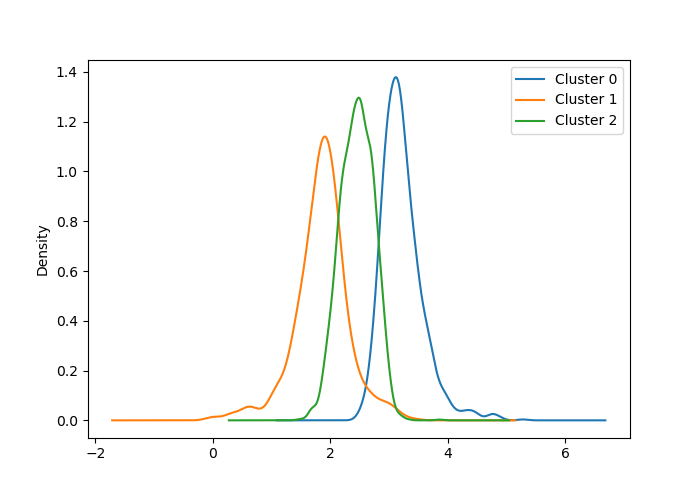
\includegraphics[width=\linewidth]{logqta_km.png}
        \caption{Distributions of \emph{logQta}}
        \label{fig:logqta}
    \end{subfigure}
    \begin{subfigure}{0.49\textwidth}
        \centering
        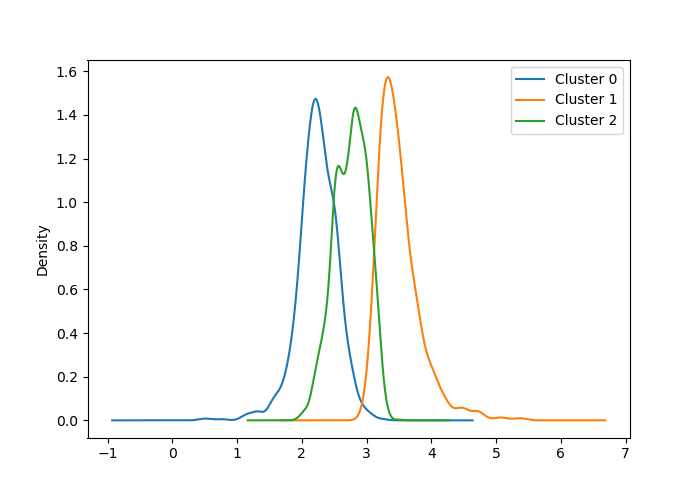
\includegraphics[width=\linewidth]{logspent_km.png}
        \caption{Distribution of \emph{logSpent}}
        \label{fig:logspent}

    \end{subfigure}
        \begin{subfigure}{0.49\textwidth}
        \centering
        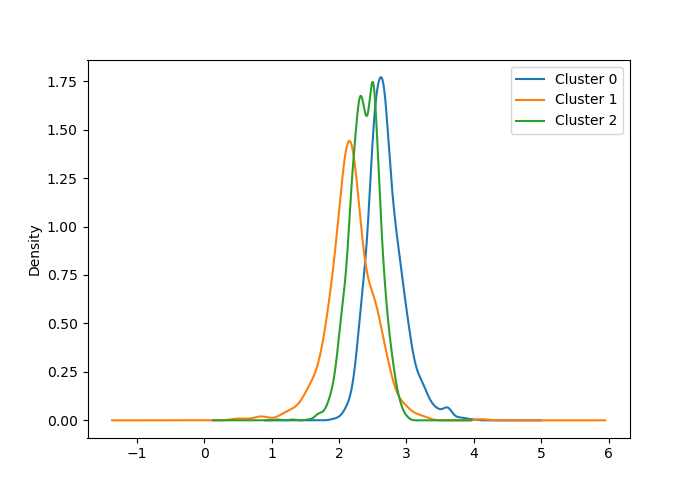
\includegraphics[width=\linewidth]{logavgbv_km.png}
        \caption{Distribution of \emph{logAvgBasksValue}}
        \label{fig:logavgbv}
    \end{subfigure}
        \begin{subfigure}{0.49\textwidth}
        \centering
        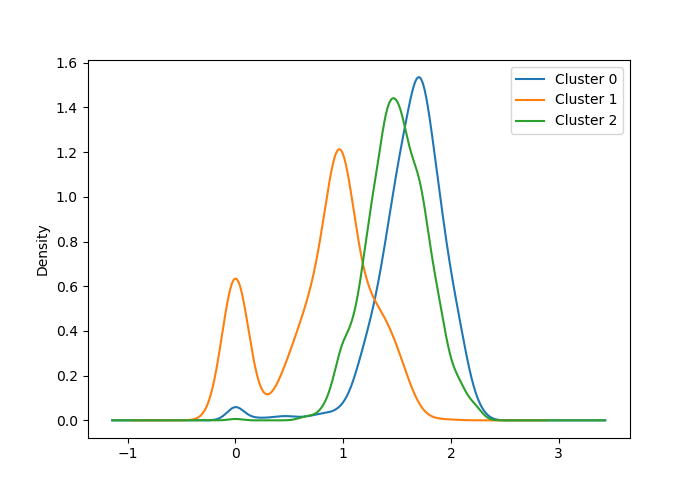
\includegraphics[width=\linewidth]{qta_entr_km.png}
        \caption{Distribution of \emph{QtaEntr}}
        \label{fig:qtaentr}

    \end{subfigure}
        \begin{subfigure}{0.49\textwidth}
        \centering
        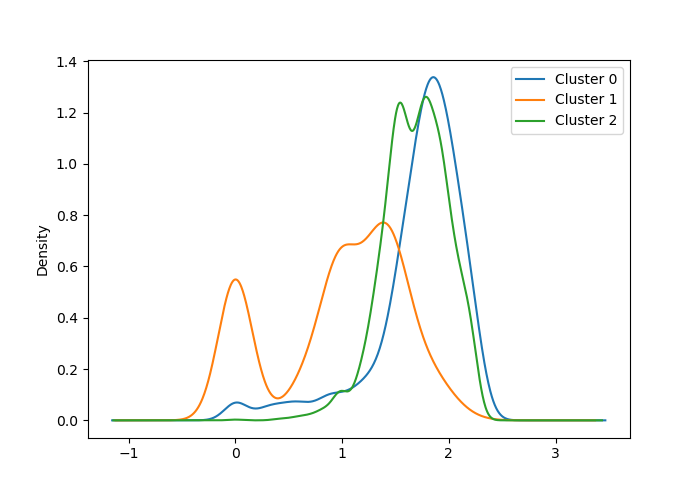
\includegraphics[width=\linewidth]{tp_entr_km.png}
        \caption{Distribution of \emph{TPEntr}}
        \label{fig:tpentr}
    \end{subfigure}
    \caption{Distribution of some attribute based partitioned with respect the clusters}
\end{figure}
\newpage
\subsection{Hierarchical clustering}
Different kinds of algorithm are used: \emph{Complete Link}, \emph{Single Link}, \emph{Ward} and \emph{Centroid}. The CPCC coefficient are respectively 0.57, 0.68, 0.47 and 0.77 meaning that the best results are obtained with \emph{Single Link} and \emph{Centroid}. By looking at the dendogram, if we cut the tree by selecting two clusters we see that the vast majority of the data fall into a single cluster leaving the last merge between a large cluster and a small one, in some cases even a singleton. The most \emph{balanced} result is obtained with the \emph{Ward} method though it has the lowest CPCC.

\begin{figure}[h!]
    \centering
    \begin{subfigure}{0.49\textwidth}
        \centering
        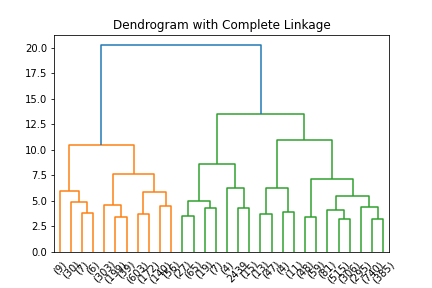
\includegraphics[width=0.9\linewidth]{c_link.png}
        \caption{\emph{Complete Link}}
        \label{fig:clink_img}
    \end{subfigure}
    \begin{subfigure}{0.49\textwidth}
        \centering
        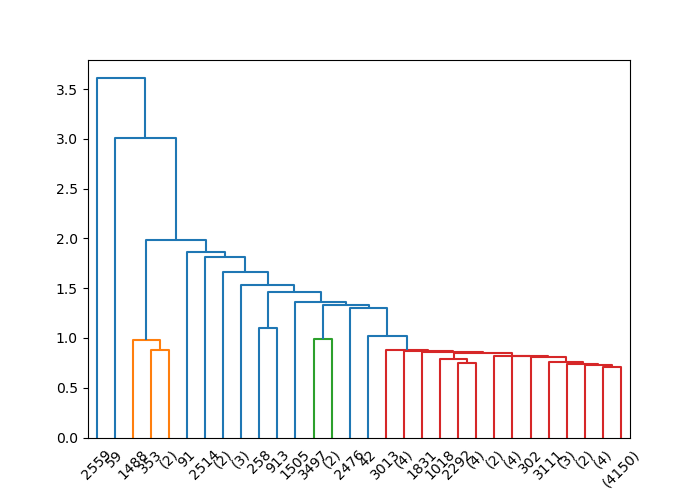
\includegraphics[width=0.9\linewidth]{s_link.png}
        \caption{\emph{Single Link}}
        \label{fig:slink_img}
    \end{subfigure}
    \begin{subfigure}{0.49\textwidth}
        \centering
        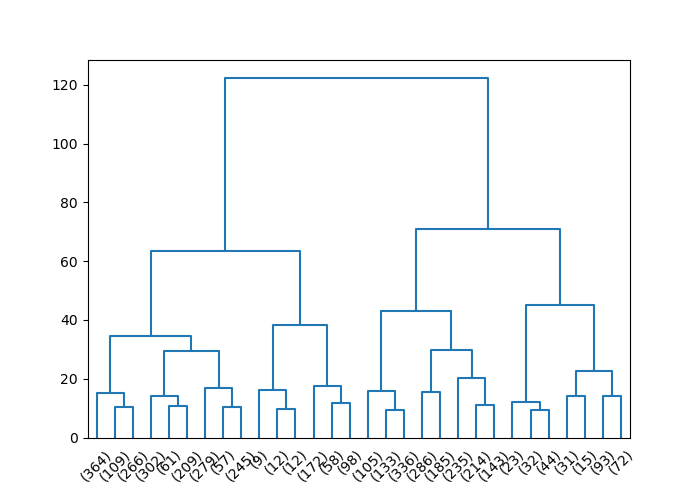
\includegraphics[width=0.9\linewidth]{ward.png}
        \caption{\emph{Ward}}
        \label{fig:ward_img}
    \end{subfigure}
    \begin{subfigure}{0.49\textwidth}
         \centering
         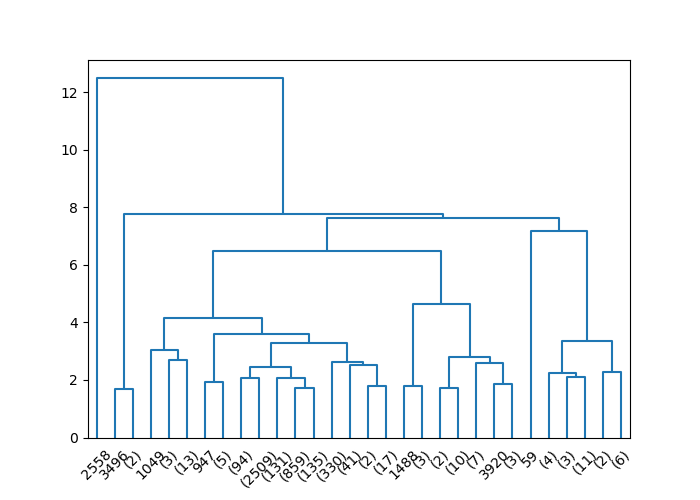
\includegraphics[width=0.9\linewidth]{centroid.png}
         \caption{\emph{Centroids}}
         \label{fig:centr_img}
     \end{subfigure}
    \label{fig:dendograms}
\end{figure}

\subsection{DBSCAN}
The dataset doesn't look suitable for DBSCAN since it is a large and dense area surrounded by a set of noise points. With different combination of \emph{eps} and \emph{MinPts} the algorithm is able to find more clusters (up to 10, including noise points, with \emph{eps} equal to 0.3 and \emph{MinPts} equal to 5), those clusters have ad small size compared to the central one which lead us to think that aren't representative. For a given value of \emph{MinPts} the selection of \emph{eps} was made by checking the \emph{Knn} distance with \emph{K} equal to \emph{MinPts}.

\begin{figure}[ht]
    \centering
    \begin{subfigure}{0.46\paperwidth}
        \centering
        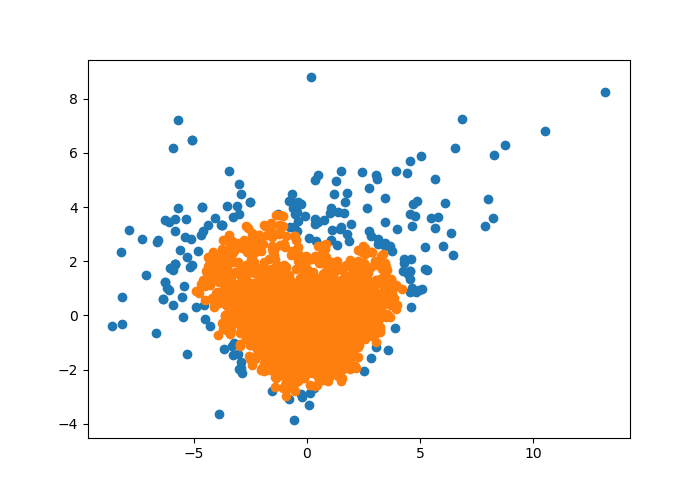
\includegraphics[width=0.9\linewidth]{dbscan.png}
        \caption{\emph{DBSCAN} with \emph{eps} equal to 0.4 and \emph{MinPts} equal to 8. There is a large and dense cluster surrounded by noise points}
        \label{fig:dbscan_good}
    \end{subfigure}
    \begin{subfigure}{0.45\paperwidth}
        \centering
        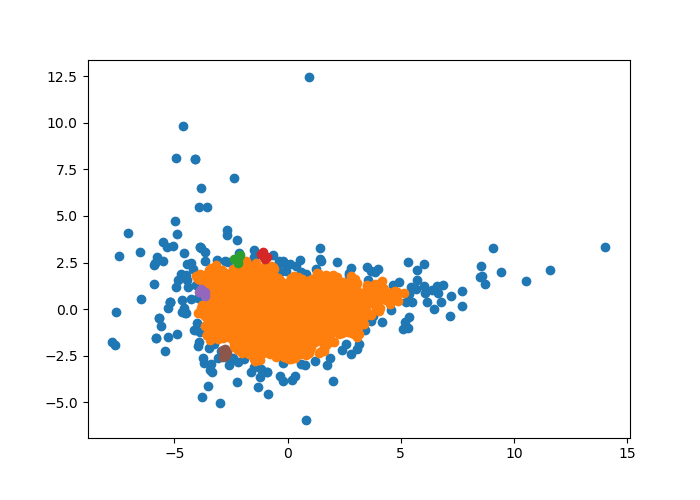
\includegraphics[width=0.9\linewidth]{dbscan_bad.png}
        \caption{\emph{DBSCAN} with \emph{eps} equal to 0.3 and \emph{MinPts} equal to 5. There is still a large and dense cluster surrounded by noise point but a large number a clusters are presents. Those clusters are really small compared to the central one.}
        \label{fig:dbscan_bad}
    \end{subfigure}
    \caption{}
    \label{fig:dbscan}
\end{figure}
\end{document}


 